\documentclass{standalone}
\usepackage{tikz}
\usetikzlibrary{3d,arrows, calc, backgrounds, petri, positioning, shadows, shapes}


\tikzset{
	persp/.style={scale=3.0,x={(-0.8cm,-0.4cm)},y={(0.8cm,-0.4cm)}, z={(0cm,1cm)}},
	points/.style={fill=white,draw=black,thick}
	grid/.style={very thin,gray},
	axis/.style={->,ultra thick},
	cube/.style={thick, fill=black!15,opacity=0.5},
	cube hidden/.style={dashed},
	block/.style={
		rectangle, rounded corners,
		draw=black!80,
		fill=black!10, fill opacity=0.5,
		text=black!90, text opacity=1.0,
    text height=1.5ex,
    text depth=.25ex,
    text width=6em,
    text centered
	}
}

\tikzstyle{class}			=[rectangle, rounded corners, draw=black, fill=blue!40, drop shadow, text centered, anchor=north, text=white,    text width=3cm]
\tikzstyle{module}		=[rectangle, rounded corners, draw=black, fill=red!40, 	drop shadow, text centered, anchor=north, text=white,    text width=3cm]
\tikzstyle{component}	=[rectangle, rounded corners, draw=black, fill=green,   drop shadow, text centered, anchor=north, text=black!90, text width=3cm]
\tikzstyle{single}		=[text height=1.5ex, text depth=0.25ex]
\tikzstyle{double}		=[text height=4.0ex, text depth=2.75ex]
\tikzstyle{triple}		=[text height=6.5ex, text depth=5.25ex]
\tikzstyle{quadru}		=[text height=9.0ex, text depth=7.75ex]
\newcommand*{\rootPath}{../}

\begin{document}
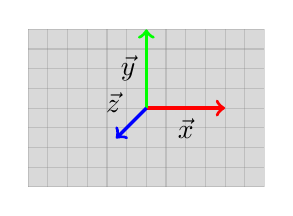
\begin{tikzpicture}
	
	\coordinate	(Ocube)	at (0,0,0);
	\coordinate	(Xcube)	at (1,0,0);
	\coordinate	(Ycube)	at (0,1,0);
	\coordinate	(Zcube)	at (0,0,1);
	\coordinate (A) at ($(Ocube)-1.5*(Xcube)-1.0*(Ycube)$);
	\coordinate (B) at ($(Ocube)+1.5*(Xcube)-1.0*(Ycube)$);
	\coordinate (C) at ($(Ocube)-1.5*(Xcube)+1.0*(Ycube)$);
	\coordinate (D) at ($(Ocube)+1.5*(Xcube)+1.0*(Ycube)$);

	\fill[black!50,opacity=0.3] (A)--(B)--(D)--(C)--cycle;
	\foreach \t in {-1.50,-1.25,...,+1.50} { \draw[black!50,opacity=0.3] ($(Ocube)+\t*(Xcube)-1.0*(Ycube)$)--($(Ocube)+\t*(Xcube)+1.0*(Ycube)$); }
	\foreach \t in {-1.00,-0.75,...,+1.00} { \draw[black!50,opacity=0.3] ($(Ocube)-1.5*(Xcube)+\t*(Ycube)$)--($(Ocube)+1.5*(Xcube)+\t*(Ycube)$); }

	\draw[->,very thick,red]		(Ocube)--(Xcube)	node[black,midway,below]			{$\vec x$};
	\draw[->,very thick,green]	(Ocube)--(Ycube)	node[black,midway,left]				{$\vec y$};
	\draw[->,very thick,blue]		(Ocube)--(Zcube)	node[black,midway,above left]	{$\vec z$};
\end{tikzpicture}
\end{document}
